\documentclass{standalone}
\usepackage{pgfplots}
\pgfplotsset{compat=newest}

\begin{document}
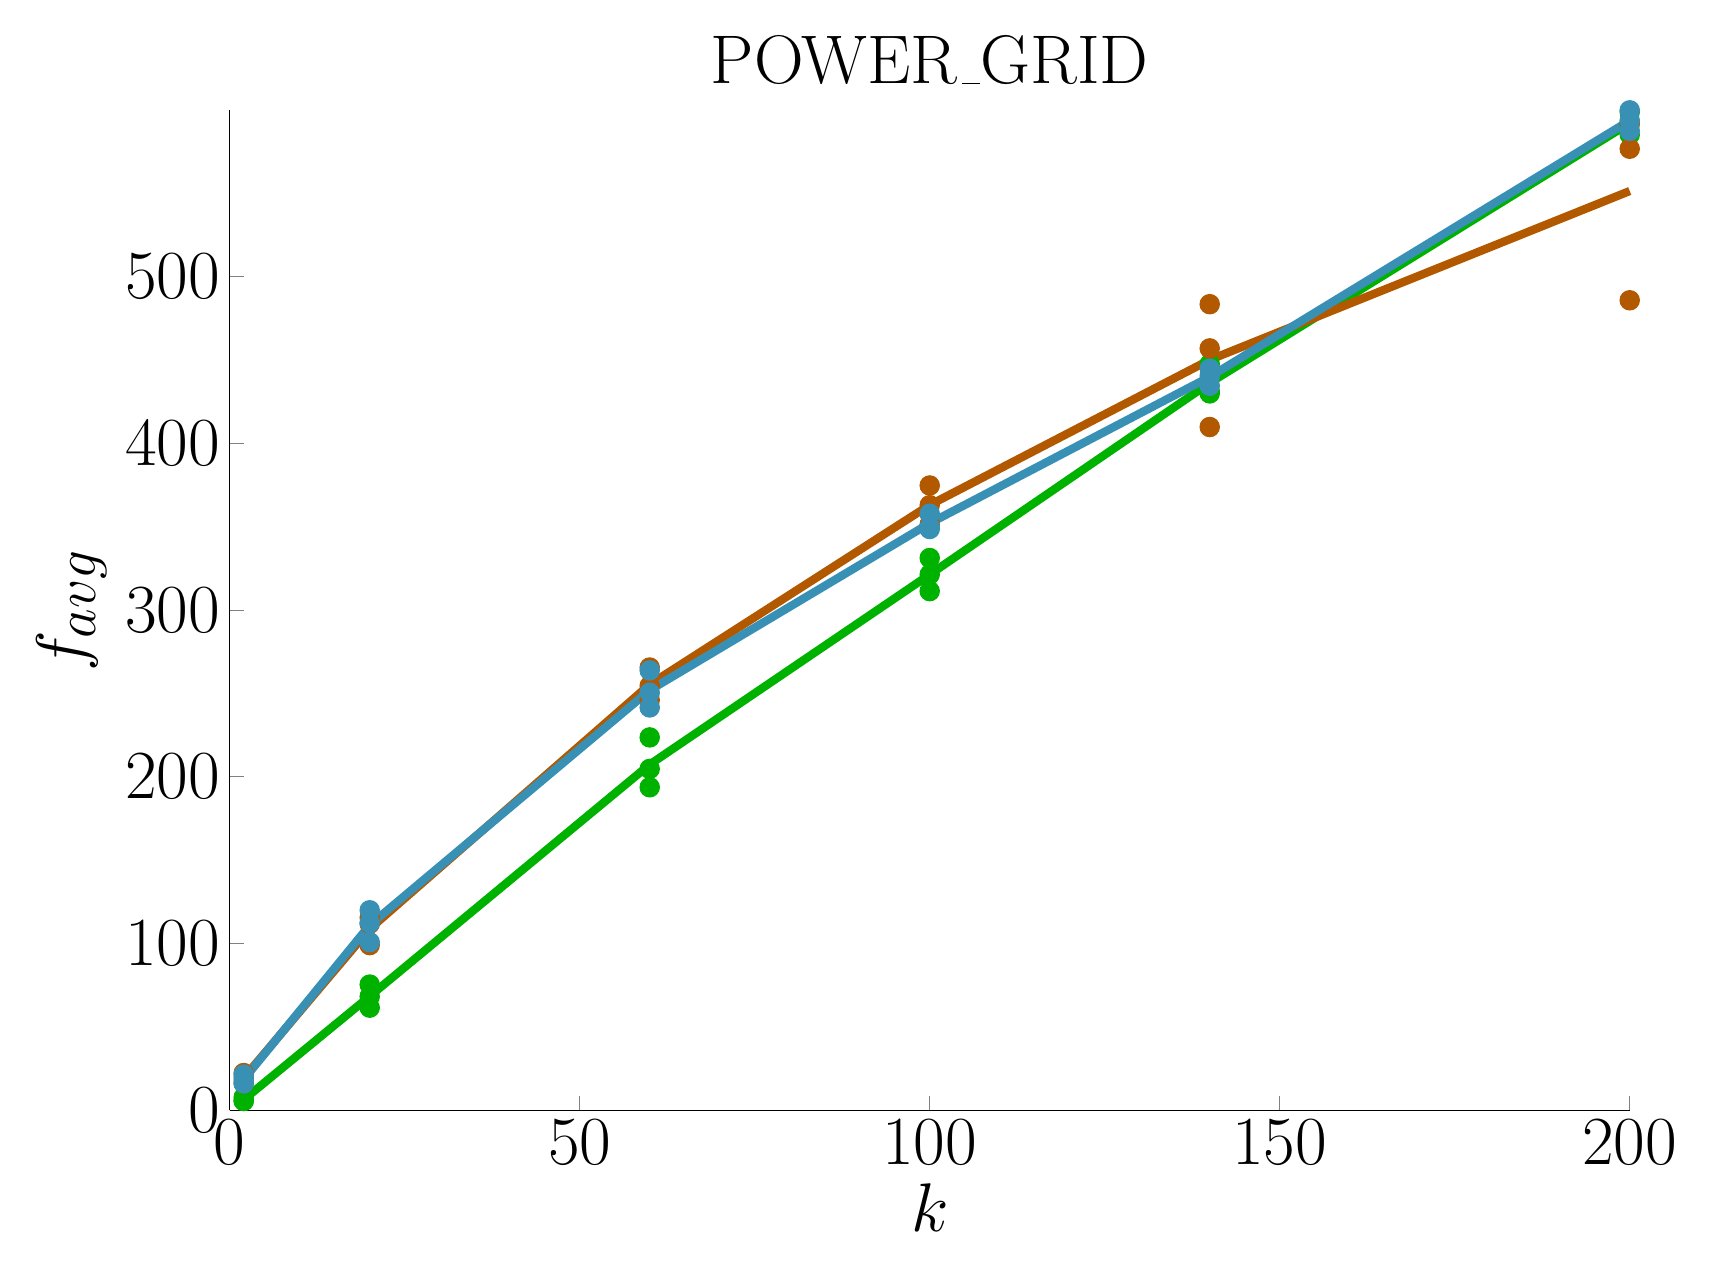
\begin{tikzpicture}

\begin{axis}[%
title style={font=\Huge},
title=POWER\_GRID,
tick label style={font=\Huge},
label style={font=\Huge},
legend style={font=\Huge},
view={0}{90},
max space between ticks=50pt,
width=7in,
height=5in,
scale only axis,
xmin=0, xmax=200,
xtick={0, 50, 100, 150, 200},
xlabel={$k$},
ymin=0, ymax=599.6,
%ytick={0, 200, 400, 600, 800, 1000},
ylabel={$f_{avg}$},
major tick length=5pt,
axis lines*=left,
legend cell align=left,
clip=false]

\addplot [
only marks,
mark=*,
mark size=3.5pt,
color=green!70!black,
%solid,
%line width=2pt,
]
coordinates{
(2,5.55)(2,5.8)(2,7.8)(20,61.55)(20,68.2)(20,75.4)(60,193.7)(60,204.7)(60,223.6)(100,311.3)(100,321.3)(100,331.15)(140,429.85)(140,431.15)(140,447.45)(200,585.0)(200,592.15)(200,598.6)
};

\addplot [
only marks,
mark=*,
mark size=3.5pt,
color=orange!70!black,
%solid,
%line width=2pt,
]
coordinates{
(2,16.2)(2,19.8)(2,22.35)(20,99.05)(20,111.8)(20,115.45)(60,245.95)(60,254.5)(60,265.5)(100,351.3)(100,362.85)(100,374.65)(140,409.7)(140,456.85)(140,483.35)(200,485.7)(200,576.55)(200,591.35)
};

\addplot [
only marks,
mark=*,
mark size=3.5pt,
color=cyan!70!black,
%solid,
%line width=2pt,
]
coordinates{
(2,16.15)(2,18.05)(2,21.4)(20,100.8)(20,112.35)(20,119.95)(60,241.55)(60,250.35)(60,263.75)(100,348.55)(100,349.7)(100,357.7)(140,434.45)(140,440.3)(140,444.6)(200,587.3)(200,593.45)(200,599.6)
};

\addplot [
color=green!70!black,
solid,
line width=3pt
]
coordinates{
(2,6.38333333333)(20,68.3833333333)(60,207.333333333)(100,321.25)(140,436.15)(200,591.916666667)
};

\addplot [
color=orange!70!black,
solid,
line width=3pt
]
coordinates{
(2,19.45)(20,108.766666667)(60,255.316666667)(100,362.933333333)(140,449.966666667)(200,551.2)
};

\addplot [
color=cyan!70!black,
solid,
line width=3pt
]
coordinates{
(2,18.5333333333)(20,111.033333333)(60,251.883333333)(100,351.983333333)(140,439.783333333)(200,593.45)
};


\end{axis}
\end{tikzpicture}
\end{document}
